\chapter{Background and Related Work}
\label{chapter:related}

Image and video compression codecs belong to the family of 
streaming applications. These are applications that 
consume an input stream, perform a
set of transformations on the data, and produce an output stream.
Streaming applications operate on potentially infinite streams of data,
exhibit strong producer-consumer locality, 
and often have sustained throughput or realtime output requirements. 

Previous research includes work in modeling 
environments, stream languages, parallel computing frameworks, and 
implementation studies. Modeling environments focus on the 
expression of stream programs as block topologies
and are oriented towards rapid 
prototyping and programmer efficiency.
Stream languages have tried to expose parallelism and 
communication requirements to the compiler and improve programmer 
productivity by hiding implementation details. Parallel computing 
frameworks and implementation studies have tried to produce high 
performance parallel implementations of video codecs for specific architectures. 

My work is in the context of the StreamIt programming language, 
which tries to provide the best of all worlds: it allows  
the easy expression of streaming applications, naturally 
exposes fine-grained and coarse-grained parallelism, 
and enables a compiler to produce 
scalable parallel implementations. The summary of related work in modeling
environments, languages, and parallel frameworks mentions the 
differences that set StreamIt apart. StreamIt itself is discussed 
in the following chapter, with a description of the key 
features that embody the language's design goals. 

Relevant to all stream programming efforts is the notion of 
a \textbf{structured block diagram}. A block diagram 
illustrates the computations and flow of data through an 
application. The block diagram's purpose is to provide a clean, 
conceptual understanding
of the application's behavior, cleanly abstracting functionality 
and ignoring implementation, architecture, and performance oriented details.
Boxes represent transformations on the data in the data stream 
and arrows indicate the flow of data between functional blocks.
A sample block diagram for MPEG-2 decoding
is shown in Figure~\ref{fig:dec-without-code}\footnote{There is no
official block diagram for MPEG-2 decoding included with the 
specification, but this is a block diagram I
produced based on the specification.}. 

\begin{figure}[h]
  \begin{center}
    \includegraphics[scale=0.44, angle=0]{./decoder_without_code.eps}
    \caption{Sample block diagram for an MPEG-2 decoder.}
    \label{fig:dec-without-code}
  \end{center}
\end{figure}

\section{Modeling Environments}
\label{section:related_modeling}
There have been many efforts to develop expressive and efficient
models of computation. Ptolemy~\cite{ptolemy03overview}, GRAPE-II~\cite{grape-ii}, 
COSSAP~\cite{cossap}, and MATLAB all 
provide computing models targeted for rapid prototyping environments. 
Synchronous Dataflow~\cite{lee87static} (SDF) provides a model 
that affords benefits to efficient scheduling and 
exposes parallelism and communication. SDF represents
computation as a set of independent actors that communicate at fixed
rates~\cite{lee87static}. Real applications, such as MPEG-2 codecs,
have data transforms that dictate sets of behavior changing parameters
to other transforms. These parameters occur at irregular intervals
and interrupt the regular flow of data. For example, an MPEG-2 bitstream
updates the quantization scale code at irregular intervals.
Expressing real applications
in an SDF model requires extensions that provide dynamic communication
and out-of-band control messages. 

Synchronous Piggybacked Dataflow
(SPDF) supports control messages in the form of a global state table
with well-timed reads and writes~\cite{park99spdf2,park02spdf3}.  SPDF
is evaluated using MP3 decoding, and would also be effective for
MPEG-2 decoding.  

Ko and Bhattacharyya also extend SDF with the dynamism needed for
MPEG-2 coding; they use ``blocked dataflow'' to reconfigure
sub-graphs based on parameters embedded in the data
stream~\cite{bhatta05block} and a ``dynamic graph topology'' to extend
compile-time scheduling optimizations to each runtime
possibility~\cite{ko05dgt}. 

Neuendorffer and Lee extend SDF to
support hierarchical parameter reconfiguration, subject to semantic
constraints~\cite{neuendorffer04hierarchical}.  
These models allow reconfiguration of an actor's I/O
rates and require alternate or parameterized schedules. 

MPEG-2 encoding has also been expressed in formalisms such as Petri
nets~\cite{valero02petri} and process algebras~\cite{pelayo01rosa}.

\section{Stream Languages}

There are a number of stream-oriented languages
drawing from functional, dataflow, CSP and synchronous programming
styles~\cite{survey97}.  StreamIt is one instance of a stream-based language.
Synchronous languages which target embedded
applications include Esterel~\cite{Esterel}, Lustre~\cite{Lustre},
Signal~\cite{Signal}, Lucid~\cite{Lucid77}, and Lucid
Synchrone~\cite{Lucid-Synchrone}.  Other languages of recent
interest are Cg~\cite{cg03}, Brook~\cite{brook04},
Spidle~\cite{spidle03}, StreamC/KernelC \cite{imagine03ieee},
Occam\cite{Occam}, Parallel Haskell~\cite{ph} and Sisal \cite{sisal}.
StreamIt distinguishes itself from these languages because $(i)$
StreamIt supports (but is no longer limited to) the Synchronous
Dataflow~\cite{lee87static} model of computation, $(ii)$ StreamIt
offers a ``peek'' construct that allows an actor to inspect
an item on its input channel without consuming it, 
$(iii)$ StreamIt imposes a single-input, single-output hierarchical
structure on the stream graph, and $(iv)$ StreamIt provides the
teleport messaging feature for out-of-band communication, discussed
in depth later in Section~\ref{sec:messaging}.

\section{Parallelization Frameworks}

Video codecs have been a longtime focus of the embedded
and high-performance computing communities.  Many researchers have
developed both hardware and software schemes for
parallel video compression; Ahmad et al.~\cite{ahmad01compression} and
Shen et al.~\cite{shen94overview} provide reviews. I focus on
programming models used to implement image and video codecs on 
general-purpose hardware.

Assayad et al. present a syntax of parallel tasks, forall loops, and
dependence annotations for exposing fine-grained parallelism in an
MPEG-4 encoder~\cite{assayad05mpeg4a, assayad05mpeg4b}. A series of loop
transformations (currently done by hand) lowers the representation to
an MPI program for an SMP target.  The system allows parallel
components to communicate some values through shared memory, with
execution constraints specified by the programmer. In comparison,
StreamIt adopts a pure dataflow model while making the programming
concepts as simple as possible.

Another programming model is
the Y-Chart Applications Programmers Interface
(YAPI)~\cite{kock00yapi}, which is a C++ runtime library extending
Kahn process networks with flexible channel selection.  Researchers
have used YAPI to leverage programmer-extracted parallelism in
JPEG~\cite{kock02jpeg} and MPEG-2~\cite{dwivedi01exploring}.  

Other high-performance programming models for MPEG-2 include manual
conversion of C/C++ to SystemC~\cite{pazos04soc}, manual conversion to
POSIX threads~\cite{li05alpbench}, and custom mappings to
multiprocessors~\cite{ahmadmpeg2encoder3, iwata98coarse}.
StreamIt's focus lies on the programmability, providing an
architecture-independent representation that is natural for the
programmer while exposing pipeline and data parallelism to the
compiler.

\section{Implementation Studies}

A number of implementation studies have generated
parallel MPEG-2 decoders and encoders. Ahmad et al. have had
success with MPEG-2 decoder implementations for distributed 
memory architectures that expose parallelism at the
picture level~\cite{ahmadmpeg2encoder, ahmadmpeg2encoder2}. 
They have also developed a multiprocessor MPEG-2 encoder
which parallelizes encoding across GOPs~\cite{ahmadmpeg2encoder3}. 
Because GOPs are spread out over a video, this approach 
has high latency but is suitable for offline encoders or decoders.

Li et al. have produced ALPBench~\cite{li05alpbench}, a set of benchmarks 
that includes both an MPEG-2 encoder and decoder. Both the encoder
and decoder have been written to expose parallelism at the slice level. 
Schneider uses a VHDL-based methodology for modeling multimedia 
applications~\cite{schneider99spec} and attempts to perform spatial 
decoding in parallel with temporal decoding. 
Jacobs et al. have implemented a
pipelined MPEG-2 encoder which uses thread level parallelism and
distributes sequential stages of the MPEG-2 encoding process to 
different processors on a shared network~\cite{jacobs2005mpeg}.

These implementations are useful for describing the types of 
parallelization that work well for certain architectures.
They would be useful for benchmarking a stream language 
compiler targeted to one of their architectures.

\chapter{The StreamIt Programming Language}
\label{chapter:streamit}

StreamIt~\cite{streamitcc} is an architecture independent language
that is designed for stream programming. 
StreamIt tries to preserve the block diagram structure
in the program definition,
allowing the application
developer to express functionality with a one-to-one mapping to code.

StreamIt also makes the parallelism inherent in
a computation explicit in the program representation,
exposing relevant scheduling and communication details 
to the compiler.
This follows from the preservation of the 
block diagram structure:
each block represents an independent computation kernel which can be 
executed in parallel with all other blocks. The arrows expose all the 
communication requirements between the functional blocks
and represent FIFO-ordered communication of data over tapes. 
The programmer can focus on a clean and malleable implementation
without worrying about the specific mapping of tasks to hardware. 
The implementation is portable across a wide range of architectures
because the compiler is responsible for determining layout and 
task scheduling.

StreamIt leverages the SDF model of
computation, but also supports dynamic communication rates and
out-of-band control messages.  
Previous StreamIt publications describe the language~\cite{streamitcc}, 
compiling StreamIt programs for 
parallel architectures~\cite{gordon02asplos, thies05ppopp},
and how StreamIt enables domain-specific~\cite{agrawal05cases, lamb03pldi},
cache-aware~\cite{sermulins05lctes}, and scheduling~\cite{karczmarek:sm-thesis:2002} 
optimizations.

\section{Filters as Programmable Units}

The fundamental programmable unit in StreamIt is the \textbf{filter}.
A filter represents an independent actor with a single input and output 
data channel. Each
filter executes atomically in its own private address space. All communication with
other filters is via the input and output channels and occasionally
via control messages (see Section~\ref{sec:messaging}). The main filter 
method is the \textbf{work function} which represents a steady-state execution step.
The work function \textbf{pops} (i.e., reads) items from the filter input tape
and \textbf{pushes} (i.e., writes) items to the filter output tape. A filter
may also \textbf{peek} at a given index on its input tape without consuming the
item. 
Computations over a sliding window and permutations on input streams are simplified
by the peek construct.
The {\tt push}, 
{\tt pop}, and {\tt peek} rates are declared (when known) as part of
the work function, allowing the compiler to apply various optimizations
and construct efficient execution schedules. 

\begin{figure}[h]
  \begin{center}
    \begin{minipage}{3in}
      \begin{small}
        \begin{verbatim}
int->int filter DivideBy(int divisor) {
    work pop 1 push 1 {
        push(pop()/divisor);
    }
}
        \end{verbatim}
      \end{small}
    \end{minipage}
  \end{center}
  \caption{Simple division filter.}
  \label{fig:divide}
\end{figure}

The simplest filter definition used in the MPEG-2 decoder
is given as an example in 
Figure~\ref{fig:divide}. This filter consumes a stream whose elements 
are of type {\tt int} and produces a stream of the same type.
This filter's output is simply its input divided by the divisor parameter
given at instantiation time. (The current version of the StreamIt compiler 
resolves all such parameters at compile time, allowing additional 
optimizations.)

The parameterization of filters allows for multiple instantiation
with different configurations, facilitating malleability and code reuse.
Shown in Figure~\ref{fig:zigzag-filter} is a filter that 
performs an arbitrary reordering on a set of $N$ elements
according to an ordering matrix. Each instantiation of the filter specifies the
matrix dimensions, as well as the desired ordering. The {\tt Order} parameter defines the
specific scan pattern that a filter instance will use.
In the example the filter performs the zigzag descrambling necessary to 
reorder the input stream in the decoder (see Section~\ref{sec:MPEGspatial}). 
The zigzag scrambling in the encoder
reuses this filter with a different {\tt Order} matrix.

\begin{figure}
  \begin{center}
    \begin{minipage}{3in}
      \begin{small}
        \begin{verbatim}
int->int filter ZigZag(int N, 
                       int[N] Order) {
    work pop N push N {
        for (int i = 0; i < N; i++)
            push(peek(Order[i]));
        for (int i = 0; i < N; i++)
            pop();
    }
}

int[64] Order =
    {00, 01, 05, 06, 14, 15, 27, 28,
     02, 04, 07, 13, 16, 26, 29, 42,
     03, 08, 12, 17, 25, 30, 41, 43,
     09, 11, 18, 24, 31, 40, 44, 53,
     10, 19, 23, 32, 39, 45, 52, 54,
     20, 22, 33, 38, 46, 51, 55, 60,
     21, 34, 37, 47, 50, 56, 59, 61,
     35, 36, 48, 49, 57, 58, 62, 63};
        \end{verbatim}
      \end{small}
    \end{minipage}
  \end{center}
  \caption{Zigzag descrambling filter.}
  \label{fig:zigzag-filter}
\end{figure}


In this example, the input matrix is represented as a unidimensional
stream of elements. The filter peeks the elements and
copies them to the output stream in the specified order. Once all the
DCT coefficients are copied, the input stream is deallocated from the
tape with a series of pops. The input and output buffers
are represented implicitly. It has been shown that this program representation
enables the automatic generation of vector permutation 
instructions~\cite{yelick04msp}.

\section{Hierarchical Streams}

In StreamIt, the application developer focuses on the hierarchical
assembly of the stream graph and its communication topology, rather
than the explicit management of the data buffers between filters.
StreamIt provides three hierarchical structures, 
shown in Figure~\ref{fig:containers},
for composing filters into larger stream graphs.  
A \textbf{pipeline} places components in series,
connecting the output from one filter to the input of the subsequent filter. A
\textbf{splitjoin} places filters in parallel and specifies both a distribution of data and
a gathering of data. There is also a \textbf{feedback loop}
hierarchy which is not needed 
for MPEG-2 decoding or encoding. 
All 
hierarchical stream components are parameterizable.
Because each hierarchical component 
itself consists of a single
input and output, hierarchical components may be
treated like filters and used inside of
increasingly larger stream hierarchies.

\begin{figure}[h]
  \center{
    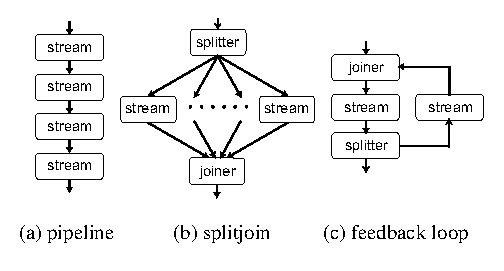
\includegraphics[scale=1.2, angle=0]{./constructs-eg.eps}
    \vspace{-12pt}
 	\caption{Hierarchical streams in StreamIt.}
 	\label{fig:containers}
  }
\end{figure}

\subsection{Pipeline}
A pipeline is a single input to single output parameterized
stream. It composes streams in sequence, with the output of
each filter connected to the input of the 
subsequent filter. 
An example pipeline from the
MPEG-2 decoder appears in Figure~\ref{fig:decoder-pipeline}.
This pipeline decodes blocks, compressed as described in Section~\ref{sec:MPEGspatial}. 
The first filter zigzag reorders the input
stream, preparing the data for the inverse quantization and
IDCT. The output of the filter is consumed by a stream named {\tt
IQuantization} that performs the inverse quantization, and produces an
output stream that is in turn consumed by another stream that performs 
\texttt{Saturation}, which produces output consumed by the \texttt{MismatchControl} filter,
which in turn passes the data to the \texttt{2D\_iDCT} and one final \texttt{Saturation}.

\begin{figure}
  \begin{center}
    \begin{minipage}{3.5in}
      \begin{small}
        \begin{verbatim}
int->int pipeline BlockDecode() {
  int[64] Order = {...};
  add ZigZagUnordering(64, Order);
  add InverseQuantization();
  add Saturation(-2048, 2047);
  add MismatchControl();
  add 2D_iDCT(8); // 8x8 2D IDCT
  add Saturation(-256, 255);
}
        \end{verbatim}
      \end{small}
    \end{minipage}
  \end{center}
  \caption{Example pipeline.}
  \label{fig:decoder-pipeline}
\end{figure}

The {\tt add} keyword in StreamIt instantiates a specified stream
using any given arguments. The {\tt add} statement may only appear in
non-filter streams.  In essence, filters are the leaves in the
hierarchical construction, and composite nodes in the stream graph
define the encapsulating containers. This allows modular design
and development of large applications, thereby promoting
collaboration, increasing code reuse, and simplifying debugging.

\subsection{Splitjoin}
A splitjoin processes data in parallel, specifying both a data
scattering and gathering. In a
splitjoin, the \textbf{splitter} distributes the data and the
\textbf{joiner} gathers the data. A splitter is a specialized
filter with a single input and multiple output channels. On every
execution step, it can distribute its output to any one of its
children in either a \textbf{duplicate} or a \textbf{roundrobin} manner.  A
duplicate splitter (indicated by \texttt{split duplicate}) replicates
incoming data to each stream connected to the splitter.  A
roundrobin splitter (indicated by {\tt split
roundrobin($w_1,\ldots,w_n$)}) distributes the first $w_1$ items to
the first child, the next $w_2$ items to the second child, and so
on.  The splitter counterpart is the joiner. It is a specialized
 filter with multiple input channels but only one output channel. 
The joiner gathers data from its predecessors in a roundrobin manner to
produce a single output stream.

An example splitjoin is shown in Figure~\ref{fig:spatialdecode}, which
encapsulates the spatial decoding necessary in the MPEG-2 decoder. Its input
consists of a stream of data interleaving coded block coefficients and 
coded motion vectors. The roundrobin splitter separates the data,
passing block coefficients to the \texttt{BlockDecode} component and 
motion vectors to the \texttt{MotionVectorDecode} component. Note that this splitjoin
treats the \texttt{BlockDecode} pipeline, previously defined in Figure~\ref{fig:decoder-pipeline},
as a primitive element. The roundrobin joiner remerges the data streams. In this case,
the \texttt{MotionVectorDecode} filter consumes two elements for every element it produces,
so the joiner has a different join rate than the splitter. Splitters and joiners
may be expressed at the natural granularity of the data and need not have matched rates.

\begin{figure}
  \begin{center}
    \begin{minipage}{3in}
      \begin{small}
        \begin{verbatim}
int->int splitjoin SpatialDecoding {
    split roundrobin(64, 16);
    add BlockDecode();
    add MotionVectorDecode();
    join roundrobin(64, 8);
}
        \end{verbatim}
      \end{small}
    \end{minipage}
  \end{center}
  \caption{Example splitjoin.}
  \label{fig:spatialdecode}
\end{figure}

\section{Execution Model}

A StreamIt program can be abstracted as a directed graph in which a node is
either a filter, splitter, or joiner, and an edge represents a data channel.
When a node executes, it removes data stored on incoming data channels and
generates output on outgoing data channels. A single node execution atomically 
transfers the smallest amount of data across the node. 

An execution schedule is an ordered list of 
executions of nodes in the graph. 
StreamIt programs have two execution schedules: one for initialization and 
one for steady state behavior. The initialization schedule primes the 
input channels, allowing filters with peeking to execute the first instance
of their work functions. The steady state schedule leaves exactly the 
same number of data items on all channels between 
executions of the schedule. Figure~\ref{fig:steady-state} shows an example
of a steady state execution schedule for a pipeline. 

\begin{figure}
  \begin{center}
    \includegraphics[scale=0.7, angle=0]{./scheduling_example.eps}
    \caption{Sample steady state execution schedule for a pipeline.}
    \label{fig:steady-state}
  \end{center}
\end{figure}

The StreamIt compiler can derive steady-state schedules at compile time
for portions of a stream graph with statically determined data rates. 
Nodes with dynamic rates require additional runtime semantics but the 
conceptual model is still expressed in terms of static execution schedules.
A more detailed explanation of the execution model and
program scheduling in StreamIt can be found 
in~\cite{karczmarek:sm-thesis:2002, streamit-lang-ref}.

\section{Teleport Messaging}
\label{sec:messaging}
A notoriously difficult aspect of stream programming, from both a
performance and programmability standpoint, is reconciling regular
streaming dataflow with irregular control messages.  While the
high-bandwidth flow of data is very predictable, realistic
applications such as MPEG also include unpredictable, low-bandwidth
control messages for adjusting system parameters (e.g., desired
precision in quantization, type of picture, resolution, etc.).

For example, the inverse quantization step in the decoder uses a
lookup table that provides the inverse quantization scaling factors.
However, the particular scaling factor is determined by the stream
parser. Since the parsing and inverse quantization tasks are logically
decoupled, any pertinent information that the parser discovers must be
forwarded to the appropriate streams. It can not easily be intermingled
with the block coefficients that the parser outputs because
control parameters occur at irregular intervals. 
In StreamIt, such communication issues are resolved conveniently
using \textbf{teleport messaging}~\cite{thies05ppopp}.

\begin{figure}
  \begin{center}
    \begin{minipage}{4.25in}
      \begin{small}
        \begin{verbatim}
01 void->void MPEGDecoder {
02   ...
03   portal<InverseDCQuantizer> p;
04   ...
05   add Parser(p);
06   ...
07   add InverseDCQuantizer() to p;
08   ...
09 }
10 int->int filter Parser(portal<InverseDCQuantizer> p) {
11   work push * {
12     int precision;
13     ...
14     if (...) {
15       precision = pop();
16       p.setPrecision(precision) [0:0];
17     }
18     ...
19   }
20 }
21 int->int filter InverseDCQuantizer() {
22   int[4] scalingFactor = {8, 4, 2, 1};
23   int    precision = 0;
24   work pop 1 push 1 {
25     push(scalingFactor[precision] * pop());
26   }
27   handler setPrecision(int new_precision) {
28     precision = new_precision;
29   }
30  }
        \end{verbatim}
      \end{small}
    \end{minipage}
  \end{center}
  \caption{Messaging example.}
  \label{fig:messaging}
\end{figure}

The idea behind teleport messaging is for the {\tt Parser} to change
the quantization precision via an asynchronous method call, where
method invocations in the target are timed relative to the flow of
data in the stream (i.e., macroblocks). As shown in
Figure~\ref{fig:messaging}, the {\tt InverseDCQuantizer} declares a
message handler that adjusts its precision (lines 27-29). The {\tt
Parser} calls this handler through a {\it portal} (line 16), which
provides a clean interface for messaging.  The handler invocation
includes a range of latencies {\tt [min:max]} specifying when the
message should be delivered with respect to the data produced by the
sender.

Intuitively, the message semantics can be understood as tags
attached to data items.  If the {\tt Parser} sends a message to
a filter downstream (i.e., in the same direction as dataflow) with a
latency $k$, then conceptually, the filter tags the items that it
outputs in $k$ iterations of its work function. If $k=0$, the data
produced in the current execution of the work function is tagged. The
tags propagate through the stream graph; whenever a filter inputs an
item that is tagged, all of its subsequent outputs are also
tagged. The message flows through the graph until the first tagged data
item reaches the intended receiver, at which time the message handler is
invoked immediately 
after\footnote{This appeared as ``immediately before'' in the 
original version of the PPoPP
2005 paper, but has since been updated.} the execution of the work function in the
receiver.  In this sense, the message has the semantics of traveling
``with the data'' through the stream graph, even though it 
need not be implemented this way.

The intuition for upstream messages is somewhat similar. Namely,
imagine a feedback loop connecting the downstream sender with the
upstream message receiver. The downstream filter uses the loop to send
tokens on every iteration, and the upstream filter checks the values
from the loop before each of its executions. If the value is non-zero,
it is treated as a message, otherwise the token is ignored. In this
scenario, the upstream message is processed immediately before it
generates data that the sender will consume in $k$ of its own
iterations.

Teleport messaging avoids the muddling of data streams with
control-relevant information. Teleport messaging thus separates the
concerns of the programmer from the system implementation,
thereby allowing the compiler to deliver the message in the most
efficient way for a given architecture. In addition, by exposing the
exact data dependencies to the compiler, filter executions can be
reordered so long as they respect the message timing.  Such reordering
is generally impossible if control information is passed via global
variables.

Teleport messaging is similar to the SDF extensions described
in Section~\ref{section:related_modeling}. However, control messages in StreamIt are more
expressive because they allow upstream messages,
adjustable latencies, and more fine-grained delivery (i.e., allowing multiple execution
phases per actor and multiple messages per phase).

\section{Prework Declarations}

Many filters require initial data processing before entering a 
steady-state execution pattern.
For instance, an exponentially weighted average might generate 
its initial value using many data items on its first execution, 
but only consume a single item per subsequent execution. 
StreamIt supports this by allowing a {\tt prework} keyword to 
specify a work function that gets executed once before the 
regular work function. 

The MPEG-2 decoder requires such a filter immediately before outputting a decoded
picture sequence. As explained in Section~\ref{subsection:pic_org}, the decoder 
must reorder pictures from their coded order to their temporal order. 
The pseudocode shown in Figure~\ref{fig:reorder_pseudocode} 
explains conceptually how to reorder
the pictures to their temporal order. 
This pseudocode is easily implemented using a filter with a prework declaration as 
written in Figure~\ref{fig:picture_reorder}.

\begin{algorithm}
\SetLine
store the first (I) picture in a delayed picture buffer\;
\ForEach{picture}{
  \eIf
    {the picture is a B-picture}
    {output immediately}{output the picture in the delayed picture buffer and store the current picture into the buffer}
}
\caption{Pseudocode for picture reordering in the decoder.}
\label{fig:reorder_pseudocode}
\end{algorithm}

\begin{figure}
  \begin{center}
    \begin{minipage}{4.5in}
      \begin{small}
        \begin{verbatim}
int->int filter PictureReorder(int picture_size) {
    int[picture_size] databuffer;
    int next_picture_type;

    prework pop datarate {
        for (int i = 0; i < datarate; i++)
            databuffer[i] = pop();
    }

    work pop datarate push datarate {
        if (next_picture_type == B_PICTURE) { 
            // B-picture is next
            for (int i = 0; i < datarate; i++)
                push(pop());
        } else {
            // I or P picture is next
            for (int i = 0; i < datarate; i++) {
                push(databuffer[i]);
                databuffer[i] = pop();
            }
        }     
    }

    handler setPictureType(int _next_picture_type) {
        next_picture_type = _next_picture_type;
    }
}
        \end{verbatim}
      \end{small}
    \end{minipage}
  \end{center}
  \caption{Sample filter with prework declaration.}
  \label{fig:picture_reorder}
\end{figure}

\section{Dynamic Rates}

\begin{figure}
  \begin{center}
    \begin{minipage}{3.5in}
      \begin{small}
        \begin{verbatim}
int->int filter RunLengthDecoder {
    work pop 2 push * {
        int itemQuantity = pop();
        int itemValue = pop();
        for (int i = 0; i < itemQuantity; i++)
            push(itemValue);
    }
}
        \end{verbatim}
      \end{small}
    \end{minipage}
  \end{center}
  \caption{Sample filter with dynamic rate declaration.}
  \label{fig:runlength-decode}
\end{figure}

Not all filters are amenable to static (initialization-time) work rate declarations. 
For example, filters which implement entropy coding/decoding schemes, 
such as Huffman coding,
will have an input / output ratio that is data dependent. Support for these
dynamic rate filters is provided by letting a wildcard {\tt *} symbol indicate an unknown rate.
A simple example is a run length decoder, shown in Figure~\ref{fig:runlength-decode}. Note that for
most dynamic rate filters, there are usually at least two equally reasonable formulations, either a static input and dynamic output rate or a dynamic input and static output rate.

\section{Functions}
StreamIt currently supports external functions and \textbf{helper} 
functions which facilitate modularity and code reuse. 
External functions typically come from a math library and 
examples used in the compression implementations are {\tt round}, 
and {\tt floor}. Helper functions are limited in scope to the 
filter in which they are defined, and are important for the same 
reasons as in procedural languages. They are particularly useful 
as a means to breakup code within filters which represent  
particularly complex computations that are not easily subdivided. 
Large filters responsible for complicated actions such as motion 
prediction or estimation rely heavily on helper functions to 
improve code readability by abstracting functionality.